\documentclass[11pt]{article}

\usepackage{lineno}

\usepackage{tikz}
\usetikzlibrary{shapes, arrows.meta, positioning}

\usepackage{makecell}
\usepackage{charter}
%\usepackage{euler}
\usepackage{inconsolata}
\usepackage{xcolor}
\usepackage[alternateNonterms]{ottalt}
\usepackage{amsmath,amsthm}
\usepackage{geometry}
\usepackage{graphicx}
\usepackage{tikz}
\usetikzlibrary{positioning,calc,3d,backgrounds}

% \usepackage{bm} % bold tt font in math mode

\geometry{margin=1in}

\inputott{formalism-commands}

\renewcommand{\ottkw}[1]{\textbf{\texttt{#1}}}

\newtheorem{definition}{Definition}

%\renewcommand{\ottcom}[1]{\textit{#1}}

%% \newcommand{\ottnt}[1]{\ensuremath{mathit{#1}}}
%% \newcommand{\ottmv}[1]{\ensuremath{\mathit{#1}}}
%% \newcommand{\ottkw}[1]{\ensuremath{\mathbf{#1}}}
%% \newcommand{\ottcom}[1]{{#1}}
%% \newcommand{\ottsym}[1]{{#1}}

\begin{document}

\author{Matthew A. Hammer}
\title{The Extended Adapton Recipe:
  \\
  \emph{Demanded Computation Graphs\\
  within\\
  Symbolic Space and Time}
}

\maketitle

\linenumbers

\section{Introduction}

A computer program has the \emph{potential} to be \textbf{incremental} if
rerunning it on similar inputs results in similar steps, and similar
outputs.
%
A \emph{fully-realized} incremental program is one where the observed
behavior is consistent with a simple, redundancy-having computer program,
but where the redundant work for similar steps is
avoided, somehow (often using some space), making it more efficient to compute in time.

The space consumed by an incremental program can store anything useful
to save time later, and often employs techniques that involve
memoization (function caching) and/or dynamic dependency graphs.
%
Adapton gives a recipe for \textbf{\emph{general-purpose incremental
  computation}} that employs its own variation of these techniques,
and hides them under a special set of programming-language-level
abstractions.
%
\begin{itemize}
\item ``\textbf{general-purpose}'' here means we care about programs
  with \emph{general recursion, over general-purpose data structures}
  with or without mutation and cycles (as opposed to a more restricted
  domain-specific language), and
  
\item ``\textbf{incremental}'' here means two complementary things at once:
  \begin {itemize}

  \item that the \textbf{program's input mutates incrementally} by the
    ambient editor program or user, in arbitrary change batches (more than one, generally), and 
    
  \item that the \textbf{program's output is demanded incrementally}
    by that ambient editor.
  \end{itemize}
\end{itemize}

\noindent
Adapton is a \emph{PL recipe}: a recipe for programming language
design and implementation.
%
It affects the \emph{programming model} exposed to the
programmer, as well as the \emph{runtime system} used by the
language's implementation.
%
Like any other such recipe, it is intended to be useful for a PL
research or engineering team interested in adding a certain kind of
flavor to their language.
%
One purpose of this document is to describe this flavor, and the
recipe behind it, to a broader audience than past publications have
reached.

This recipe maps a purely functional fragment of this team's PL into
another PL fragment that is both incremental and stateful, enriching
the original (subset of the) source PL with read and write operations
on global (and symbolically named) state:

\begin{center}
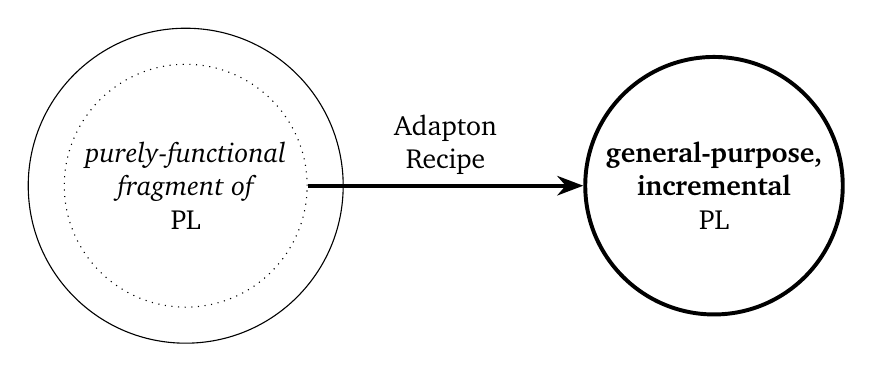
\begin{tikzpicture}[node distance=3.5cm, every node/.style={draw, align=center}]

  % Left outer blob
  \node (outerblob) [circle, minimum size=4cm] {};
  
  % Left inner blob
  \node (innerblob) [circle, minimum size=2.5cm, dotted] at (outerblob.center) {\it purely-functional\\\it fragment of\\ PL};

  % Right blob
  \node (rightblob) [circle, minimum size=2.5cm, right=of innerblob, line width=0.5mm] {\bf general-purpose,\\\bf incremental\\ PL};

  % Arrow with text
  \draw[->,  line width=0.5mm, >=Stealth] (innerblob) -- node[midway, above, draw=none] {Adapton\\Recipe} (rightblob);

\end{tikzpicture}
\end{center}

\noindent
By employing these special primitives, the program or library
expresses dependencies between inputs and outputs, reading the former
and writing the later, and Adapton hides the complexity of
representing and maintaining these various (read, write,
and~\emph{demand}) dependencies.

Behind the scenes, Adapton's recipe provides the \textbf{demanded computation graph} (DCG),
including the semantics for the graph components'
memoization and change propagation\footnote{
In a sense, Adapton enriches the existing (CBV or CBN)
\emph{evaluation strategy} of a PL with an additional dimension of
evaluation that requires a persistent a graph representation of the
program's past behavior.
%
In this presentation of the recipe, we focus on a CBV host language.
%
Past presentations used call-by-push-value (CBPV) which avoids the
choice between CBV and CBN by subsuming both; however, a CBPV
presentation can be confusing for newcomers, so we use CBV here.
}.

In this graph-based strategy, there's an ambient memory (global state)
for communicating values between different points of incremental
space-time, based on symbolic names whose definitions persist across
distinct incremental runs.
%
These symbols name the program's individual steps and datums in a way
that identifies their ``change positions'' symbolically.
%
This level of indirection turns out to be critical for efficient
incremental responses to changes.

Unlike prior versions of Adapton (see PLDI 2014 and OOPSLA 2015), this
\emph{extended} recipe embraces the idea of \emph{naming distinct
moments of time}, not just space, and permitting multiple versions of
this named past or future to coexist and reuse each other's redundant
graphical structures.
%
This new recipe subsumes earlier work, and presents the key ideas in a
single unified documented that is hopefully just as approachable, or
more approachable, than the original works.

\paragraph{Purpose of this document.}
%
The purpose of this document is to communicate the \emph{Extended Adapton Recipe} (EAR) in a way that's useful for\begin{itemize}
\item[(a)] PL researchers that are curious about DCGs and/or Adapton,
\item[(b)] language engineers with control over some host PL and an interest in making a subset of that PL into an ``incremental PL'', and
\item[(c)] users of this recipe, trying to create programs or libraries that use it, in whatever domain excites them most.
\end{itemize}

The first two groups use formal semantics as mathematical tools for communication, as does this document.
%
For the third group, the document will provide example programs with technical illustrations of
their evaluation in the formal semantics, and thus their ``behind the scenes'' behavior in terms of the DCG.

Note to draft reader: There is a pending implementation of this formal
semantics (including DCGs), and sections about it will also be added to the document
when they are ready for that. For now, the document focuses on the
\emph{formal semantics} of the recipe, and less so on any specific
\emph{implementation} of it.
  
\paragraph{Formal semantics for the recipe.}
%
Programs in this recipe have a pair of closely-related formal semantics: a
\emph{reference dynamics} that affords a limited form of incremental
reuse, and a \emph{graphical dynamics} that that is arguably more practical
and more incremental.

While the graphical dynamics describes demanded computation graphs, the
reference dynamics describes a more limited flavor of caching that is
intolerant of most effects, except for the effect of updating the
cache with otherwise-pure computation results.

The role of the reference dynamics is to \begin{itemize}
  \item[(1)] introduce the ``symbolic space-time'' semantics
    of the new read and write primitives, and
  \item[(2)] capture a familar\footnote{The author believes that this form of caching is modeling something like that found in Haskell, or even in NIX, where either isolation, or freedom from most changes (a form of purity), is required to reuse a subcomputation}, but also \emph{limited}
    form of caching that lacks dependence graphs.
\end{itemize}

The reference dynamics gives a basis for comparison with the graphical dynamics, and its increased complexity of rules.
    %
    It acts a specification for the input-output behavior we expect in our (more complex) graphical dynamics,
    and our meta theory will\footnote{Pending work.} aim to prove that the graphical dynamics is consistent with the reference semantics, and vice-versa.

\paragraph{Organization.}
This document is organized as follows:

\begin{itemize}

\item Section \ref{sec:collections} introduces the recipe's approach to programming with collection-based data structures like sequences, sets and finite maps.  The concepts introduced here are used in subsequent section's program examples.
  
\item Section \ref{sec:symbolic-space-and-time} introduces the idea of symbols and their possible program syntax.  We introduce the idea of the ``symbolic store'' used by the reference semantics.  The graphical semantics builds on these ideas and adds the concept of recording evaluation traces for these store effects.
  
\item Section \ref{sec:programs} gives some prototypical syntax
  extensions for working with symbolic space and time.
  %
  This section gives just enough detail to
  formalize the pair of dynamics (reference and graphical) in
  subsequent sections.
  %
  In practice,
  the new syntax for \ottkw{put}, \ottkw{get}, and \ottkw{force} may
  repurpose some existing syntax in the host PL, rather than use these
  particular keywords.  

\item Section \ref{sec:reference-dynamics} presents the reference dynamics.

\item Section \ref{sec:graphical-dynamics} presents the graphical dynamics.

\item Section \ref{sec:from-scratch-consistency} presents a meta theory
  about the pair of theories, for reference and graphical dynamics.
  %
  It claims that each derivation in one corresponds
  to at least one derivation in the other.  Because the reference
  dynamics enforces a strict notion of reuse, this claim implies that
  the graphical semantics is always ``from-scratch consistent'' with
  full re-evaluation.

\item Note to (draft) reader: There is a pending implementation.  Once more
  complete, sections about that would include a description of it, and
  an experimental evaluation with practical time and space
  measurements.
  
\end{itemize}

\newpage

\section{Incremental Collections}
\label{sec:collections}

We introduce the recipe's approach to collections like sequences,
sets, and finite maps based on the concept of \emph{harmonious trees},
a term of art that we introduce for the first time here, based on
intuitions and related definitions developed in prior work.

\subsection{Harmonious binary trees}

The recipe uses \textbf{binary trees} of a certain flavor to represent
each each collection type (set, partial map, or sequence).
%
Other tree arities are possible too, using more general definitions
and algorithms, but in this recipe, we focus on binary trees for
simplicity.

\begin{definition}[Harmious tree representation]
  Given a set of mathematical structures~$\mathcal{S}$ (like
  sequences, sets or finite maps of some certain element types) we say
  that binary tree representation~$\ottkw{tree}$ is \emph{harmonious}
  if it enjoys two properties:
\begin{itemize}  

\item \textbf{balance}: For each structure $S \in \mathcal{S}$, the
  corresponding tree $T = \ottkw{tree}(S)$ consists of \emph{balanced
  binary nodes}: each binary node has left and right subtrees are
  within some constant factor of each other, specific to the function~\ottkw{tree}.

\item \textbf{change stable}: similar mathematical structures $S_1,
  S_2 \in \mathcal{S}$ correspond to similar binary trees $T_1 =
  \ottkw{tree}(S_1)$ and $T_2 = \ottkw{tree}(S_2)$, with many
  identical subtree structures.  That is, if $S_1$ and $S_2$ are
  related by small change, then $T_1$ and $T_2$ should also be
  relatable with a small change.

\end{itemize}

\end{definition}

The rest of the recipe's approach to collection-based algorithms
relies on this property for each binary tree, regardless of
whether it's representing a sequence, a set or a finite map.
%
In the remainder of this section, we focus on sequences and their
representations as binary trees.

\subsection{Incremental sequences}

Mathematically, a sequence is a monoid.  As commonly found in
functional programming, we use this relationship as an approach to
representing sequences.
%
These consist of immutable sequences, like in functional programming,
but also sequences that can change from moment to moment.

In data structure terms, a \emph{monoid} is an inductive (tree-shaped)
structure that represents a sequence of data elements with an associative ``append'' operation.
%
It has three forms:

\begin{itemize}
\item The \textbf{singleton data} form carries a value of some data type that is common to the entire monoid (e.g., ``integer'', ``database record'', etc.); these elements carry the relevant ``data'' of the monoid structure.
\item The \textbf{binary node} form of two monoid structures (e.g., $L + R$), which sends this pair into a third monoid representing their being appended; this form reflects the choices of how to combine/divide within the monoid sequence structure.
\item A special \textbf{empty element}, (e.g., $0$) which ``cancels'' the binary operation by ``serving as its identity element'' (meaning that $0 + R = R$ and $L + 0 = L$ holds for all $L$ and $R$).
\end{itemize}

These forms permit a program to ``generate'' the monoid structure for
some relevant sequence of elements, in preparation for doing something
else with that sequence that involves each element, such as
determining the max element, the min element, the median element, or
even sorting it upon demand into a new, output sequence.
%
In the remainder of this section, we work towards that final example
(demand-driven sorted output sequence), building the needed components
in stages.

\subsection{Monoid generation}

Given a sequence of elements, there are many possible ways to generate a monoid.
%
For instance, a linked list is a kind of monoid structure, but it
doesn't meet either condition that we require for binary trees, as its
only a pathological kind of binary tree (totally imbalanced, and thus
not change stable either).

There are many algorithms that could generally produce acceptable
binary trees, but the recipe embraces one that uses psuedo-random
decisions based on the relative position of each element in the input
sequence.  As we show through experimentation (and argue by reference
to earlier work that established a similar approach), the recipe's
\texttt{Seq} trees provide both balance and change stability, as
required.

XXX

to do

\subsection{Monoid reduction}

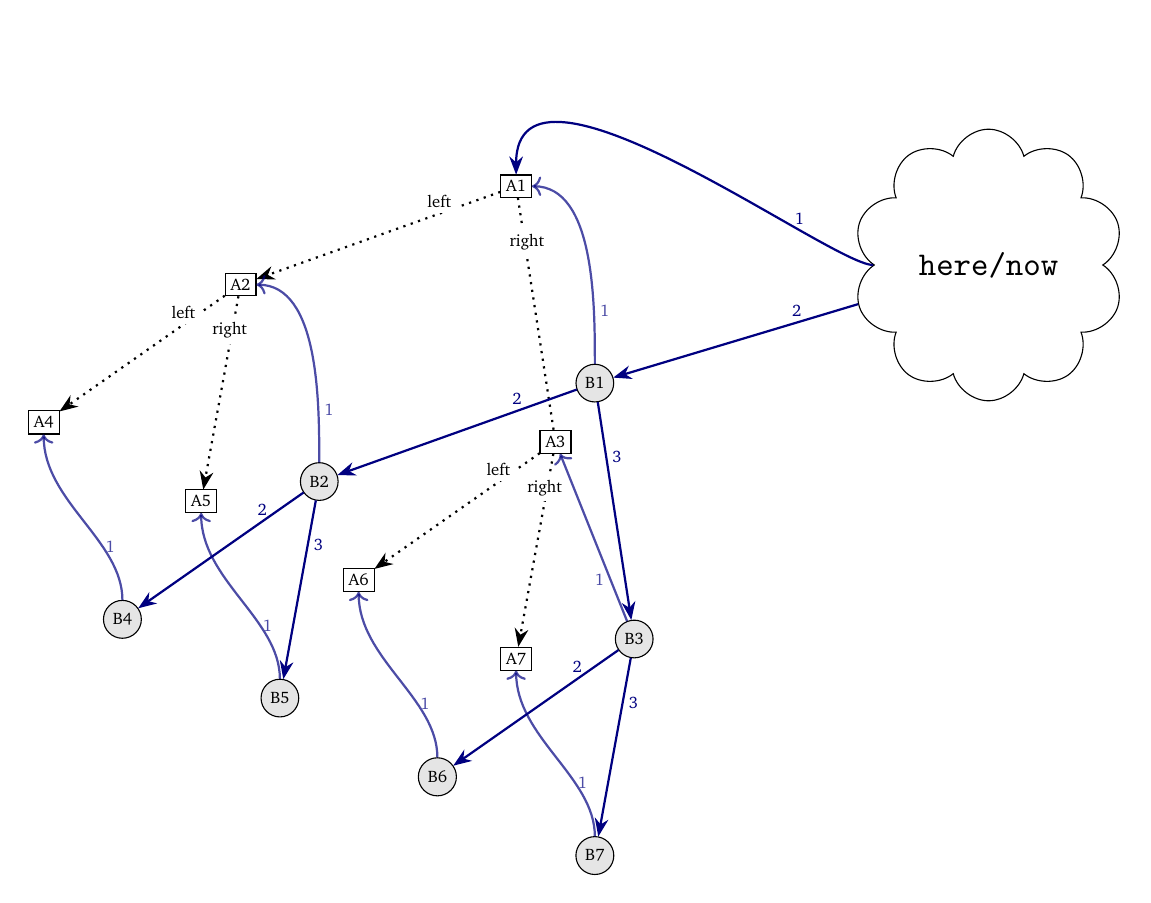
\begin{tikzpicture}[scale=2.0, every node/.style={draw, scale=0.6},
  root/.style={xshift=2cm},
  layerA/.style={yslant=-0.5, xslant=0.5, xshift=-1cm},
  layerB/.style={yslant=-0.5, xslant=0.5, yshift=-1cm},
  pointer/.style={->, thick, >=Stealth, dotted},
  connection/.style={->, thick, color=blue!50!black, opacity=0.7},
  thunk/.style={circle, draw, fill=white!80!gray},
  edge/.style={->, thick, >=Stealth, blue!50!black},
  edgeNum/.style={near start, above, draw=none},
  fieldLabel/.style={near start, above, draw=none, fill=white},
]

  \begin{scope}[root]
    \node[scale=2.0, cloud] (here-now) at (0,0) {\texttt{here/now}};
  \end{scope}
  
% Layer A: Tree A
  \begin{scope}[layerA]
  \node (A1) at (0,0) {A1};
  \node (A2) at (-1,-1.5) {A2};
  \node (A3) at (1,-1.5) {A3};
  \node (A4) at (-1.5,-3) {A4};
  \node (A5) at (-0.5,-3) {A5};
  \node (A6) at (0.5,-3) {A6};
  \node (A7) at (1.5,-3) {A7};

  \draw[pointer] (A1) -- (A2) node[fieldLabel]{left};
  \draw[pointer] (A2) -- (A4) node[fieldLabel]{left};
  \draw[pointer] (A2) -- (A5) node[fieldLabel]{right};
  \draw[pointer] (A1) -- (A3) node[fieldLabel]{right} -- (A6) node[fieldLabel]{left};
  \draw[pointer] (A3) -- (A7) node[fieldLabel]{right};
\end{scope}

% Layer B: Tree B
  \begin{scope}[layerB]
  \node[thunk] (B1) at (0,0) {B1};
  \node[thunk] (B2) at (-1,-1.5) {B2};
  \node[thunk] (B3) at (1,-1.5) {B3};
  \node[thunk] (B4) at (-1.5,-3) {B4};
  \node[thunk] (B5) at (-0.5,-3) {B5};
  \node[thunk] (B6) at (0.5,-3) {B6};
  \node[thunk] (B7) at (1.5,-3) {B7};

  \draw[edge] (B1) -- (B2) node[edgeNum] {2};
  \draw[edge] (B2) -- (B4) node[edgeNum] {2};
  \draw[edge] (B2) -- (B5) node[edgeNum,right] {3};
  \draw[edge] (B1) -- (B3) node[edgeNum,right] {3};
  \draw[edge] (B3) -- (B6) node[edgeNum] {2};
  \draw[edge] (B3) -- (B7) node[edgeNum,right] {3};
\end{scope}

% Connections between layers
\draw[connection] (B1) .. controls +(up:0.5cm) and +(right:0.5cm) .. (A1) node[edgeNum,right] {1};
\draw[connection] (B2) .. controls +(up:0.5cm) and +(right:0.5cm) .. (A2) node[edgeNum,right] {1};
\draw[connection] (B3) -- (A3) node[edgeNum,left] {1};

\draw[connection] (B4) .. controls +(up:0.5cm) and +(down:0.5cm) .. (A4) node[edgeNum] {1};
\draw[connection] (B5) .. controls +(up:0.5cm) and +(down:0.5cm) .. (A5) node[edgeNum] {1};
\draw[connection] (B6) .. controls +(up:0.5cm) and +(down:0.5cm) .. (A6) node[edgeNum] {1};
\draw[connection] (B7) .. controls +(up:0.5cm) and +(down:0.5cm) .. (A7) node[edgeNum] {1};


% edges
\draw[edge] (here-now) .. controls +(left:1cm) and +(up:1cm) .. (A1) node[edgeNum] {1};
\draw[edge] (here-now) -- (B1) node[edgeNum] {2};
\end{tikzpicture}


\section{Symbolic Space and Time}
\label{sec:symbolic-space-and-time}

This Adapton recipe uses the notion of ``symbols''.
%
Earlier Adapton publications called these identifiers ``names'', and
the role and purpose is the same here: to name distinct ``positions''
within the changing data structures, and also the changing DCG living
behind the scenes.

Informally, these symbols (or ``names'') identify distinct positions
in space, and distinct steps in time, in a way where ``similar''
evaluations will use ``similar'' names for ``similar'' purposes.
%
In the reference semantics, there is no DCG and the symbols help the
program identify distinct memory cells at distinct moments in time.
%
At each such position in space and time, there may be a stored cell
that contains a non-thunk value or a thunk:


\ottgrammartabular{\ottStore}
\ottgrammartabular{\ottcell}
\ottgrammartabular{\ottStoreValueOption}

Each store~$[[Store]]$ is a finite map (a partial map) that sends each space-time pointer~$[[pp]]$
defined by the program to a stored cell~$[[cell]]$.
%
Non-thunk cells hold values.

Each thunk cell stores a triple that includes the current space, the thunk body, and the evaluation cache.
%
The thunk's space~$[[Space]]$ corresponds to the current
space when the thunk was defined, but can be changed by the thunk's body during
evaluation, if necessary.

In UNIX terms, this initial space is akin to the initial ``working
directory'' used by a UNIX program when it starts; as with UNIX
programs, these thunks can create subspaces (akin to UNIX
subdirectories) and/or may go to other already-existing spaces.
%
Section~\ref{sec:refsem-navigation} describes the interaction of
programs and space-time in the reference dynamics.

The cache of each thunk cell~$[[StoreValueOption]]$ has one of two states:
Empty cache ($[[empty]]$) or
filled cache ($[[(Store, v)]]$).
%
The filled cache state records a store snapshot~$[[Store]]$
corresponding to the store \emph{just before} that thunk last ran,
it records the result value~$[[v]]$ of that last run.

\paragraph{Aligned stores.}

The notion of cache reuse within the reference semantics requires that
the current store~$[[Store2]]$ be an ``aligned extension'' of the store
snapshot~$[[Store1]]$ from when the thunk last ran.

The relation~$[[Store1 <= Store2]]$ formalizes this relationship as a
partial order defined inductively over the stores, as follows:

\[
\begin{array}{ll}\scalebox{1.5}{
\boxed{
  [[Store1 <= Store2]]
}}
&
\text{``Store $[[Store2]]$ is an aligned extension of store~$[[Store1]]$''}
\end{array}
\]

\begin{mathpar}
  \drule{AXXempty}
  \drule{AXXbinary}
  \drule{AXXcell}
  \drule{AXXcache}
\end{mathpar}
\[
\drule{AXXequiv}  
\]

\noindent
Whenever this relation fails to hold for a pair of stores, it means
that one or more cells are not part of an aligned extension, and the
following relation will hold instead:

\[
\begin{array}{ll}
  \scalebox{1.5}{
\boxed{
  [[Store1 </= Store2]]}
}
&
\text{``Store $[[Store2]]$ is \textbf{not} an aligned extension of store~$[[Store1]]$''}
\end{array}
\]

\begin{mathpar}
  \drule{NAXXfocus}
  \drule{NAXXchanged}
  \drule{NAXXforgot}
\end{mathpar}

\noindent
(\textbf{Note to draft reader}:
It remains to prove that these relations are negations of each other,
and that the alignment relation is a partial order.
%
It may also be interesting or useful to state the alignment relation
independently of the structure of the stores.)

\paragraph{Reference dynamics versus graphical dynamics.}
%
This aligned-store extension relationship permits no
mutable effects other than thunk evaluation, making it considerably
more limited than the graphical semantics.

In contrast to the reference semantics, the graphical structure of the
DCG can identify fine-grained opportunities for reuse, and if
necessary, repair them to be aligned with the current program state.
%
The cost to create the DCG is a constant factor per store action,
whereas the reference semantics either foregoes caching, or requires
creating and comparing snapshots for alignment.

%
The graphical dynamics is motivated by the need to avoid these various
impracticalities.
%
However, we wish to retain the reference semantics as a reasoning tool,
as it is comparatively simpler than the graphical semantics,
and yet enjoys a close formal correspondance with it.
%
Indeed, we intend to prove (proof pending) that every derivation in
the reference semantics has a corresponding derivation in the
graphical semantics, and vice versa.

In addition to the impractical nature of store snapshots, the other practical
difference between these two dynamics is that the \emph{size of the
derivation} in the graphical dynamics will always be similar to, or
smaller than, the smallest corresponding one in the reference
dynamics, and sometimes \emph{much} smaller.
%
This compression in derivation size comes from the ability of the
graph to always facilitate equivalent, or more, patterns of cache reuse.

The next subsections introduce the formal syntax for symbols, spaces, moments (of time) and pointers.
%
These concepts, along with program syntax~(Section~\ref{sec:programs}) are common to both dynamics.

\subsection{Symbols}
\label{sec:symbols}

A symbol is a
unique identifier, determined dynamically by a running program, or fed
as part of its input, or some combination of those two methods.
%
When used to name something, like a specific datum or sub-computation,
the incremental program also implicitly says when and where to reuse
it later, as the program re-executes incrementally.

\ottgrammartabular{
  \otts
}

Each symbol $\ottnt{s}$ is made of one or more literals,
combined with binary composition operators.
%
The details of these literal symbols (numbers, strings, etc) and
binary composition operators is inconsequential to the rest of the
Adapton recipe.  Any conventions that make sense for the ambient host PL will work.

Here, we assume three binary composition forms that get overloaded: the
dot operator usually reserved for field access, and the minus operator
usually reserved for arithmetic, and the application form usually reserved for function calls.
%
We overload these forms to construct symbol trees.
%
The intention of minus and dot here are to mimick common composit
names in UNIX, where dashes and dots are common word separators.
%
We use the application form to indicate sub-spaces and sub-moments.

\subsection{Symbolic pointers.}
\label{sec:symbolic-pointers}

Each program or library that uses this recipe
defines a system of symbolic names for space and time.
The details of this system are program/library-specific, and the
design of the recipe itself affords a chance to compose distinct systems to
create larger ones.
Essentially, the chance to compose distinct systems stems from the choice of moments
and space to each be \emph{nestable} (or \emph{fractal}) in nature.

\nolinenumbers
\ottgrammartabular{
  {\makeLineNumber\stepLineNumber} \ottSpace
  \\
   {\makeLineNumber\stepLineNumber} \ottMoment
  \\
   {\makeLineNumber\stepLineNumber} \ottp
  \\
   {\makeLineNumber\stepLineNumber} \ottpp
  \\
  {\makeLineNumber\stepLineNumber} \ottd
}
\linenumbers

Programs using this recipe have control over space and time in ways
that ordinary programs do not.
%
One aspect of this control is the distinction between
\emph{space-time} and \emph{time-space} regions of the store, which are complementary in
the recipe.
%
The storage used by the program distinguishes these regions as follows.
%
Space-time ($[[d = st]]$) holds data that ``is'' part of a moment.
By contrast,
time-space ($[[d = ts]]$) holds data that is ``becoming'' part of a moment.

When the program navigates time, this data that is ``becoming'' part
of the target moment transitions atomically into what ``is'' at that
target moment where the program arrives.
%
Sections~\ref{sec:refsem-navigation} and~\ref{sec:refsem-undelay}
define the reference semantics for navigating space and time, including
how time navigation ``buffers'' updates in a separate region.


\section{Programs}
\label{sec:programs}

The Adapton recipe we present here assumes a CBV host language, with a
pre-existing model of common language features, such as recursive data
types, recursive functions, pattern matching, and other details.
%
To this host language, the recipe adds a handful of special value
forms and special expression forms.

\paragraph{Thunks as values.}
In contrast to earlier CBPV-based presentations that fused all thunks
with the ambient global state (PLDI 2014 and OOPSLA 2015), here we
assume ordinary thunks exist in the host language already and we treat
them as a distinct, ordinary value type.
%
Because they are central to the special new forms, we illustrate their
(pure) dynamics in detail, though again this dynamics is the ordinary one.

\paragraph{Value syntax.}
The recipe assumes (or adds) an ordinary notion of thunk values.
%
To this, it adds symbols, pointers, spaces and moments (See Sections~\ref{sec:symbols} and \ref{sec:symbolic-pointers}).

\ottgrammartabular{
  \ottv
}

\paragraph{Expression syntax.}

We begin by assuming usual CBV expression forms, and thunks.
%
To these forms, the Adapton recipe also adds expression forms that
affect the ambient mutable state: \textbf{put}, \textbf{get}, \textbf{force}.
%
The forms \textbf{here}, \textbf{now} and \textbf{do} help indicate
and control the current space and moment of the program, respectively.
%
Together, the current space and moment influence how the individual
cells of global state are created and accessed.

\ottgrammartabular{
  \otte
}

\ottgrammartabular{
  \ottC
  \\
  \ottCxtVerb
  \\
  \ottCxtDim
}  

\noindent
The syntax we show above is clear, but not concise.
%
To help remedy this for common situations, we introduce some syntactic sugar, as follows.

\paragraph{Do-at notation.}

The ``do-at'' notation is shorthand for the common programming idiom
of writing a thunk to the graph within a space (here,~$[[e1]]$) and then
immediately forcing it's evaluation (the body~$[[e2]]$):

\[
\begin{array}{lcl}
  [[do @e1 ({( e2 )}) ]]
  &\equiv&
  [[let x = put((e1, thunk((e2)))) in]]
  \\
  &&[[force((x))]]
\end{array}
\]

\paragraph{Do-at-within notation.}
Another common variation of this shorthand does the thunk within a
certain subspace:

\[
\begin{array}{lcl}
  [[do @e1 within e2 ({( e3 )})]]
  &\equiv&
  [[let x = put((e1, thunk((do within space ((e2))({(e3)}) )))) in]]
  \\
  &&[[force((x))]]
\end{array}
\]

\noindent
Sometimes, it can be preferable (and simpler) to reuse the same symbol
as the thunk-naming symbol to name this subspace:

\[
\begin{array}{lcl}
  [[do @within e1 ({( e2 )})]]
  &\equiv&
  [[let x = e1 in]]
  \\
  &&[[let y = put((x, thunk((do within space ((x))({(e2)}))))) in]]
  \\
  &&[[force((y))]]
\end{array}
\]

\section{Reference Dynamics}
\label{sec:reference-dynamics}

\[
\begin{array}{lc}
\scalebox{1.5}{\boxed{
  [[Store1; Path; Moment; Space |- e !! Store2; v]]
}}
&
\begin{array}{p{4in}}
  ``
  Under store~$[[Store1]]$,
  path~$[[Path]]$,
  space~$[[Space]]$,
  and
  moment~$[[Moment]]$,\\
  \hspace{3mm}~expression~$[[e]]$ evaluates fully,\\
  \hspace{6mm}~resulting in store~$[[Store2]]$ and value~$[[v]]$.
  ''
\end{array}
\end{array}
\]


\subsection{Pure thunks.}

Thunk values that are not stored are forced in the usual way:

\[
\drule{EXXthunk}
\drule{EXXforceThunk}
\]

\subsection{Symbol expressions.}

Symbols are values:

\[
\drule{EXXsym}
\]

Some expressions produce symbol trees:

\[
\drule{EXXsymMinus}
\drule{EXXsymDot}
\drule{EXXsymApp}
\]

\subsection{Putting a value into the store.}
\label{sec:refsem-get}

Put operations write to the global store.
%
There are two temporal cases: immediate in space-time, or delayed in time-space:

\[
\begin{array}{cc}
\drule{EXXputImmediate}
&
\drule{EXXputDelay}
\end{array}
\]

\noindent
%
Each value put into the store can either be a thunk or a non-thunk value.
For a thunk, the store update syntax $[[Store{pp |-> (Space, v)}]]$
means that $[[v = thunk((e))]]$ for some expression~$[[e]]$,
and this update is defined as $[[Store{pp |-> Thunk(Space, e, empty)}]]$.
Alternatively, when $[[v /= thunk((e))]]$, 
the update ignores the space~$[[Space]]$ and is defined instead as $[[Store{pp |-> NonThunk v}]]$.


\subsection{Getting a value from the store.}
\label{sec:refsem-get}

There are two cases for $\ottkw{get}$, depending on whether~$[[cell]]$ is a non-thunk value, or a thunk cell.
For the latter, the operation returns a pair that includes the space value used by the thunk (note that $[[Space1]]$, $[[Space2]]$ and $[[Space0]]$ can all be distinct).

\[
\begin{array}{cc}
\drule{EXXgetNonThunk}
&
\drule{EXXgetThunk}
\end{array}
\]

\noindent
In each \texttt{get} rule, the store access $[[Store((Space2, Moment) ^ st) = cell]]$ compares the current moment~$[[Moment]]$ to those written at the given space~$[[Space2]]$, choosing the ``latest'' cell whose moment is equal to or earlier than~$[[Moment]]$, if it exists.
It is not defined when no such moment exists.

\subsection{Forcing a thunk pointer}

There are three cases for forcing a stored thunk (pointer).
%
Recall that this makes four cases for~$\ottkw{force}$ in total,
as \rref{E-force} handles the ordinary, non-pointer case.

\begin{mathpar}
\drule{EXXemptyForce}
\drule{EXXreuseForce}
\drule{EXXredoForce}
\end{mathpar}

When stored, the thunk's cache is either empty (\rref{E-emptyForce}),
or it has a store-value pair.
%
To fill an empty cell, \rref{E-empty} evaluates the thunk body (under
the original stored space) and caches the result and initial store.

\Rref{E-reuseForce} captures the situation where that cached value was produced
under a prior store such that the current store is an aligned extension of it.
%
\Rref{E-redoForce} captures the opposite case, where the current store is not an aligned extension of the prior store.
%
As with \rref{E-emptyForce}, this rule evaluates the thunk body (under
the original stored space) and caches the result and initial store.

\subsection{Navigating space-time}
\label{sec:refsem-navigation}

There are a pair of rules for giving access to $\ottkw{here}$ and $\ottkw{now}$
as first-class space/moment values, respectively,
and four rules that permit programs to navigate through space and time,
including the creation of sub-spaces and sub-moments (\rref{E-withinSpace} and \rref{E-withinTime}).

\[
\begin{array}[t]{p{0.731in}|c|c}
  & \textbf{Space} & \textbf{Time}
  \\[2mm]
  \hline
  &&
  \\[2mm]
  \begin{tabular}[l]{l}\texttt{here},\\\texttt{now}\end{tabular}
  & \drule{EXXhere}
  & \drule{EXXnow}
  \\[2mm]
%  \hline
%  &&
%  \\[2mm]
  
  \texttt{goto}
  &
  \drule{EXXgotoSpace}
  &
  \drule{EXXgotoMoment}
  \\[2mm]
%  \hline
%  &&
%  \\[2mm]

  \texttt{within}
  &
  \drule{EXXwithinSpace}
  &
  \drule{EXXwithinMoment}
\end{array}
\]

\subsection{Navigating time: Undelay}
\label{sec:refsem-undelay}

For time navigation (\rref{E-withinTime} and \rref{E-gotoTime}),
all delayed cells in the target region of time-space are ``undelayed''
before evaluation continues at that target moment.
%
The following relation based on five rules formalizes this idea:

\begin{mathpar}
\drule{undelayXXempty}
\drule{undelayXXbinary}
\drule{undelayXXmoment}
\drule{undelayXXskipMoment}
\drule{undelayXXskipSpace}
\end{mathpar}


\section{Graphical dynamics}
\label{sec:graphical-dynamics}

\subsection{Graphs}
\label{sec:graphs}

A graph $[[Graph]]$ consists of nodes and edges.
%
The nodes in the graph correspond to the cells of the store structure in the reference semantics.
%
Each node is identified by a full pointer, and a ``meta moment'', which we explain shortly.

The edges of the graph each have a unique identifier (some natural number~$[[n]]$) and each corresponds to a store-based action performed by the program~($\ottkw{put}$, $\ottkw{get}$ or $\ottkw{force}$).
  
\ottgrammartabular{
  \ottGraph
}

%\paragraph{Graph node pointers and meta moments.}

\ottgrammartabular{
  \ottppp
}

\paragraph{Nodes.}
To distinguish different versions of a node over time,
the graphical representation introduces another dimension of time called ``meta moments''
represented by natural numbers and meta variable~$[[m]]$.
%
Each node pointer in the graph carries the meta moment for its definition, or re-definition.
%
Each time a node is updated, it's updated with an advanced meta moment that distinguishes it from earlier versions.

In a practical system, earlier versions of the same node are
``shadowed'' by later meta moments, and the shadowed versions can be
discarded, or saved, depending on other considerations.
%
We retain them here as an illustration of one possible ``lossless'' representation for a DCG in a practical system that desires that property.

For each node version, the local trace~$[[t]]$ gives a ordering to the node's immediate outgoing edges.
%
Compared to the reference semantics and its store structure, this
trace~$[[t]]$ is a practical way to fill the role played by taking
snapshots of the full store~$[[Store]]$ for each thunk's evaluation,
and caching and comparing that snapshot.
%
Instead of doing that, the graphical semantics is more incremental:
It can partially dirty and clean a thunk's edges, and in so doing, it also avoids any comparison of the entire graph
when reusing the cached values of thunks in the graph.

\ottgrammartabular{
  \ottnode
  \\
  \ottcache
  \\
  \ottt
}

\paragraph{Edges.}
Each edge~$[[ppp --A--b--> qq]]$ records an action~$[[A]]$, and
associates with it the source of the action~$[[ppp]]$ (some thunk node
in the graph) and the target of the action~$[[qq]]$ (some other node
in the graph).
%
The status~$[[b]]$ indicates whether the edge is $[[clean]]$ (aligned
with current graph) or $[[dirty]]$ (not aligned with current graph).

\ottgrammartabular{
  \ottedge
  \\
  \ottA
  \\
  \ottb
}


\paragraph{Well-formed graphs.}
To ensure that incremental evaluation always produces results
consistent with from-scratch evaluation (a form of ``incremental
correctness''), graphs must remain \textbf{well-formed}, an invariant
formally required by the dynamics.

A graph is well-formed when each evaluated node has a cached result
from some earlier run on a well-formed graph.
%
That earlier run can be very out-dated with respect to the current graph.
%
In those cases, an additional aspect of the graph being well-formed
also insists on the status of an edge be dirty whenever its truly
outdated, or depends on some edge that is, transitively.
%
The dirty status can be overly-conservative, but it must hold
transitively, in every case.

More operationally, each write effect to a graph node also traverses
the dependencies of immediately affected edges, whenever the new value
differs from the originally-observed one on such an edge.
%
A transitively affected node is either a directly affected node
itself, a node that directly forces a directly affected node, or one
that transitively forces it.

\subsection{Dirtying.}

The relations for dirtying use the idea of an ``action pattern'' that
matches certain actions, and not others:

\ottgrammartabular{
  \ottDirtyActionPattern
}

The idea is that when a $\ottkw{put}$ updates a particular pre-existing cell in the graph,
each existing action that targets that cell is either aligned or misaligned with that update.
%
The $[[misaligned(Space,v)]]$ pattern matches any action that is
misaligned with (i.e., ``inconsistent with'' or ``disequal to'') a
$\ottkw{put}$ of that space-value~$([[Space]],[[v]])$; it captures this
initial part of the dirtying traversal.

Then, beyond that first set of affected nodes, each force on any of
node with a misaligned action/edge, directly or transitively, could be
affected too.
%
The $[[forces]]$ pattern captures this second part of the dirtying
traversal.

There are six rules for dirtying: One for dirtying ``target nodes,''
and five for processing their incoming edges (dependent edges),
transitively.

\[
\begin{array}{lc}
  {\scalebox{1.5}{
  \boxed{[[Graph1 |- dirty ( DirtyActionPattern , ppp ) !! Graph2]]}}}
&
\begin{array}{p{4in}}
  ``Dirtying edges that match pattern~$[[DirtyActionPattern]]$,\\
  \hspace{4mm}~that target node~$[[pp]]$ in graph $[[Graph1]]$ yields graph~$[[Graph2]]$.''
\end{array}
\end{array}
\]

\[
\drule{dirtyNode}
\]

\noindent
\Rref{dirtyNode} uses another dirtying relation (given just below) to
process each edge in the set of edges that target the node~$[[ppp]]$.
%
The same action pattern is compared against the action on each edge.
%
In contrast to cleaning, the ordering of dirtying these edges is
inconsequential to the final output of the dirtying traversal.
%
To make the rules determinisitic, we can sort the edge identifiers by
their happenstance natural numbers.

\[
\begin{array}{lc}
  {\scalebox{1.5}{
  \boxed{[[Graph1 |- dirty ( DirtyActionPattern , t ) !! Graph2]]}}}
&
\begin{array}{p{4in}}
  ``Dirtying incoming edge set~$[[t]]$ in $[[Graph1]]$\\
  \hspace{4mm}~that match pattern~$[[DirtyActionPattern]]$ yields graph~$[[Graph2]]$.''
\end{array}
\end{array}
\]

\begin{mathpar}
  \drule{DTXXempty}
  \drule{DTXXbinary}
  \drule{DTXXalreadyDirty}
  \drule{DTXXcleanIntoDirty}
  \drule{DTXXstillClean}
\end{mathpar}

There are five rules for dirtying a set of relevant edges, expressed as a sequence~$[[t]]$.
%
Two cases express the monoidal structure of the
sequence (\rref{DT-empty, DT-binary}), and
three cases express the possible situations for dirtying each edge/action
(\rref{DT-alreadyDirty}, \rref{DT-cleanIntoDirty},
\rref{DT-stillClean}).

\Rref{DT-alreadyDirty} expresses how the dirtying algorithm ``short
circuits'' (quits early) when it encounters a dirty edge; it relies on
the graph's well-formedness to justify this behavior.
%
The graph being wellformed guarentees that the edges that the traversal
would encounter if it were to continue are already marked dirty.

\rref{DT-cleanIntoDirty} applies when the action of the edge~$[[A]]$
matches the pattern of the traversal at this
point~$[[DirtyActionPattern]]$.
%
The rule updates the edge to be~$[[dirty]]$, and it recursively
dirties any $[[forces]]$ that target the source of the edge, as they
may be affected too.
%
This recursive premise helps enforce that the graph remains
well-formed with respect to transitive $[[dirty]]$ vs $[[clean]]$ edge statuses.

\rref{DT-stillClean} applies for an edge that is clean, and whose
action~$[[A]]$ does not match the pattern~$[[DirtyActionPattern]]$;
for instance, it's common for the put edge that targets (and defines)
a thunk node to remain clean even as that node is affected by actions
it performs, like accessing cells that change.
%
This independence of the $\ottkw{put}$ stems from the definition of the
thunk being distinct from its behavior under any particular store or
graph.

\subsection{Cleaning.}

There are eight rules for cleaning: Two for cleaning nodes, and six for cleaning their traces.

\[
\begin{array}{lc}
  {\scalebox{1.5}{
  \boxed{[[Graph1; Path; Moment; m; Space |- clean(pp) !! Graph2]]}}}
&
\begin{array}{p{4in}}
  ``
  Under initial graph~$[[Graph1]]$,
  path~$[[Path]]$,
  space~$[[Space]]$,\\
  \hspace{3mm}~moment~$[[Moment]]$ and meta-moment~$[[m]]$,\\
  \hspace{6mm}~pointer~$[[pp]]$ cleans fully,
  resulting in graph~$[[Graph2]]$.
  ''
\end{array}
\end{array}
\]

While cleaning nodes, there are two cases: Nodes that are aligned
(\rref{CN-aligned}) and those that are not (\rref{CN-misaligned}):

\begin{mathpar}
\drule{CNXXaligned}
\drule{CNXXmisaligned}
\end{mathpar}

Algorithmically, the ``alignment'' of the node is a function of its trace, and is indicated by the final status of cleaning that trace under the current graph.
%
When $[[clean]]$, we say that the node is still \emph{aligned with the graph}.
Otherwise, when $[[dirty]]$, we say that the node is \emph{misaligned} with the current graph.
%
To remedy the latter situation, the cleaning algorithm replaces misaligned traces with updates ones,
based on re-evaluating the node under the current graph (see \rref{CN-misaligned}).
%

\Rref{CN-misaligned} captures the case of a misaligned node, where at least one
local edge is not cleanable because it witnesses an action with an
outdated value.
%
The judgement~$[[Graph1; Path; Moment; m; Space |- clean(t) !!
    Graph2; dirty]]$ captures this situation for a trace~$[[t]]$ that contains this edge.
%
We call this trace and its edge ``misaligned'' because they cannot be ``aligned with''
(reconciled with) the current graph.
%
In these situations, the graph node is generally misaligned with the graph as well, with an outdated value.

To clean the node, the rule replaces the old trace with an updated one
from an updated evaluation.
%
This new evaluation occurs with an advanced meta moment, and the rule
updates the trace and value for the node by including this advanced
meta moment in the new graph node pointer.
%
Each distinct meta moment in the graph corresponds to the use of this
rule, the only rule that advances it.


The following relation specifies how to clean a node's trace~$[[t]]$, either fully or partially,
thereby determining which node cleaning rule applies.

\[
\begin{array}{lc}
  {\scalebox{1.5}{
  \boxed{[[Graph1; Path; Moment; m; Space |- clean(t) !! Graph2; b]]}}}
&
\begin{array}{p{4in}}
  ``
  Under initial graph~$[[Graph1]]$,
  path~$[[Path]]$,
  space~$[[Space]]$,\\
  \hspace{3mm}~moment~$[[Moment]]$ and meta-moment~$[[m]]$,\\
  \hspace{6mm}~cleaning trace~$[[t]]$
  results in status~$[[b]]$ and graph~$[[Graph2]]$.
  ''
\end{array}
\end{array}
\]

\begin{mathpar}
\drule{CTXXempty}
\drule{CTXXbinL}
\drule{CTXXbinR}
\drule{CTXXalreadyClean}
\drule{CTXXdirtyIntoClean}
\drule{CTXXmisaligned}
\end{mathpar}

There are six rules for cleaning a trace.
%
Three cases express the monoidal structure of the
trace (\rref{CT-empty}, \rref{CT-binL}, \rref{CT-binR}), and
three cases express the possible situations for each edge/action
(\rref{CT-alreadyClean}, \rref{CT-dirtyIntoClean},
\rref{CT-misaligned}).

The three edge rules determine if a node is aligned or misaligned.
%
Each aligned edge uses one of the
two \rref{CT-alreadyClean,CT-dirtyIntoClean}.

\Rref{CT-misaligned} applies for a misaligned edge, where the action
is no longer aligned with the graph.
%
To procede with cleaning the source node~$[[ppp]]$, this misaligned edge~$[[n]]$ must be
replaced by a use of \rref{CN-misaligned}, which will replace each
immediate action of~$[[pp]]$ with an updated (aligned) action/edge.

\subsection{Graphical evaluation}

\[
\begin{array}{lc}
  {\scalebox{1.5}{
  \boxed{[[Graph1; Path; Moment; m; Space |- e !! Graph2; t; v]]}}}
&
\begin{array}{p{4in}}
  ``
  Under initial graph~$[[Graph1]]$,
  path~$[[Path]]$,
  space~$[[Space]]$,\\
  \hspace{3mm}~moment~$[[Moment]]$ and meta-moment~$[[m]]$,\\
  \hspace{6mm}~expression~$[[e]]$ evaluates fully,\\
  \hspace{9mm}~resulting in graph~$[[Graph2]]$, local trace~$[[t]]$ and value~$[[v]]$.
  ''
\end{array}
\end{array}
\]

\subsection{Putting values into the store.}

(Compared to reference dynamics, very similar, but uses dirtying for put and stores edges.)

\subsection{Getting values from the store.}

(Compared to reference dynamics, very similar, but stores edges.)

\subsection{Forcing a thunk pointer.}

There are two rules for forcing a thunk pointer in the graphical semantics.
%
Both are similar to their reference semantics counterparts; we focus on the differences.

\Rref{IE-emptyForce} handles the case where the thunk cache is empty
by evaluating the thunk (under the appropriate path and space) and
storing the resulting trace and value in the cache.

\Rref{IE-cleanForce} handles the case where the thunk cache is filled
by first cleaning the thunk node, and then accessing the aligned (up
to date) resul value from the cache.

Compared to the reference semantics, the is only one rule for a filled
cache, and this rule always applies, and cleaning always succeeds
(somehow) in updating the cache to be aligned with the current graph.
%
Sometimes, cleaning will effectively ``redo'' the thunk if needed, but
not in every case where the reference semantics falls back to a
``redo''.

\textbf{Note to draft reader}: We need an example here to help illustrate the point. Pending.

\begin{mathpar}
\drule{IEXXemptyForce}
\drule{IEXXcleanForce}
%\drule{EXXreuseForce}
%\drule{EXXredoForce}
\end{mathpar}

\subsection{Undelay.}

(Compared to reference dynamics, very similar, but uses dirtying.)

\section{From-scratch Consistency}
\label{sec:from-scratch-consistency}

Both of the following hold:
\begin{itemize}
\item[(1)] $\begin{array}[t]{lcl}
  [[Graph1; Path; Moment; m; Space |- e !! Graph2; t; v]]
  & \Rightarrow &
  \exists
      [[Store1]], [[Store2]].~~
      [[Store1 ~~ Graph1]]
      ~~\bigwedge~~ [[Store2 ~~ Graph2]]
      %\\
      %&&
  ~~\bigwedge~~ [[Store1; Path; Moment; Space |- e !! Store2; v ]]
  \end{array}$
\item[(2)] $\begin{array}[t]{lcl}
  [[Store1; Path; Moment; Space |- e !! Store2; v]]
  & \Rightarrow &
  \exists
      [[m]], [[t]],
      [[Graph1]], [[Graph2]].~~
      [[Store1 ~~ Graph1]]
      ~~\bigwedge~~ [[Store2 ~~ Graph2]]
      %\\
      %&&
  ~~\bigwedge~~ [[Graph1; Path; Moment; m; Space |- e !! Graph2; t; v ]]
  \end{array}$
\end{itemize}

\end{document}

% ------------------------------------------------------------------

\paragraph{The ambient path function.}
%
The path function~$\texttt{\textcolor{red}{<<no parses (char 2): pa***th >>}}$ is used by the \textbf{put} operation when it writes
the graph to create a \emph{global pointer symbol} from a given
\emph{local symbol value}.

Unlike the thunk body, the path function is restricted to be a pure
function that sends symbols to symbols, while performing no write or
read effects on graph itself.
%
Each write performed by the thunk body's uses this function to
localize written pointers to a specific dynamic invocation, mapping
locally-defined symbols into larger, more specific ones based on the
dynamic context that defined the path function
\footnote{
Compared to OOPSLA 2015, the recipe here refines and simplifies the
presentation of ``namespaces,'' making them into ordinary (but pure)
functions in the ambient programming language.
%
Here, we call them ``path functions'', but the role is the same.

Like in that work, the role of paths/namespaces is not evident without
worked example programs that use collection libraries to perform
incremental algorithms.
%
Without them, it's tedious to program and use these libraries in a
generic-enough way; while possible, library authors tend to reinvent
the concept of paths/namespaces in their own style, where they pollute the
library API, making it less concise and readable.
%
By including them, we make programs and libraries more concise and
uniform in their calling conventions.
}.


% ------------------------------------------------------------------

\subsection{Naming strategies and program complexity}

The initial semantics for Adapton (PLDI 2014) defined demanded
computation graphs (DCGs).  It maintained these graphs' consistency
status via dirtying and cleaning algorithms.  These algorithms
transition graph components between two possible states: potentially
inconsistent (``dirty'') and definitely consistent (``clean'').

Initially, the Adapton recipe focused on a simple cache model: A mutable
input store, created and changed by the ambient editor, and a cached DCG
whose graph components were identified and reused dynamically via hash
consing
%
\footnote{
%
%A hash is a symbolic name produced by a hash function.
%
Hash consing is the canonical way to cache data structures and avoid
allocating otherwise-equivalent, duplicate copies; it identifies shared dynamic
allocations using the hash of the allocations' written data, written
to a so-called \emph{memoization table} that tracks each unique hash
currently in use.  Initially, the Adapton recipe used this technique
to name every DCG node (excluding initial input cells), as it
identified every incremental program-allocated thunk or reference cell
with a hash of its defining data.
%
}.
%
While always ``correct'' (no name-consistency issues follow from this
naming strategy), the programmer also gets no direct control over the
name for the written pointer.

The hash-consing naming strategy is limited because hashes can be
fragile, and in data structures, they make names sensitive to
non-local changes.
%
For example, the head of a linked list has a hash that is impacted by
every element in the list, not just the meaning attached to the prefix
of the list, whatever it may be.
%
If this list is used as the intermediate data structure in a larger
incremental algorithm, reconstructing its prefix with new (hash) names
also means recomputing all downstream dependencies on this data,
eventually.
%
This example shows how hash consing insists that small changes cascade
into large ones.
%
Indeed, follow on work showed how that approach was severely limited
in many important cases (like this one), and gave a generalization
providing more precise and effective incremental behavior
\cite{ICWithNames}.

While more powerful, the drawback of this more general recipe is the
more complex programmering model.
%
% TO DO -- Cite Personal Correspondance with Yan Chen
%
To gain the extra power, programmers need to conciously choose an
``(incremental) naming strategy'' for their programs that leads to the
dynamic behavior that they desire.
%
Specifically, the programmer needs to consider their algorithm's cache
behavior across the the expected pattern of input changes and output
observations that they anticipate.
%
If that consideration is too complicated, they can always fall back to
hash consing every allocation, but to get the best behavior, that
choice often falls very short or fails entirely, as discussed.

This ``naming strategy'' design task can be complex, much like
developing an entirely new algorithm is often a complex design task.
%
However, in summary, it also seems necessary to get the best
incremental performance possible within ``interesting'' incremental programs.
%
\footnote{ There's a long-running CS joke that there are ``only''
three hard problems in all of CS: (1) Naming things (2) Cache invalidation
and (3) Off-by-one errors.  The evolution of the Adapton Recipe is about viewing (1) and (2) as two vantage points of a single,
persistent CS problem to solve.  }

\paragraph{Named writes.}
We name writes to achieve better indendepence of distinct parts of a changing data structure.
%
Each such write is identified by an input name, a programmer-chosen name, or a combination of those, as computed by the program's logic, which Adapton enhances with practical name introduction forms, like symbolic constants and binary composition.

In this approach, each ``allocation'' is a named write, and is
determined by the program input (directly or indirectly), and thus is
deterministic and even ``stable'' across similar executions.

Contrast named allocation with the usual (non-hash-consing) kind, where the outer system either makes unstrategic choices for ``fresh'' pointers, or uses a strategy that generally hinders reuse (something for GC practicality, for example).

Named allocation can create an extra logical burden for the programmer to think through, but it's also consistent with long-standing, familar practices in practical incremental systems.
%
For instance, programmers have long thought about organizing files in a directory tree such that each change independently from one another, but also reflect functional dependencies across the files too, e.g., based on re-running a tool like \texttt{make}.
%
Adapton gives a similar approach, but where the filesystem holds data values (structures), not just text or binary files, and where there is no possible way to misauthor the program (the \texttt{Makefile}) so that it fails to reflect consistent functional dependencies.

\paragraph{Restrictions on effects.}
%
Past Adapton systems restrict effects so that, despite being technically impure, programs and their graphs remain \textbf{quasi-pure} (or \emph{quasi-functional}).

Specifically, each named write in a from-scratch consistent program execution is:

\begin{itemize}
\item \textbf{unique}, meaning each named write is globally unique within the graph.
  
\item \textbf{causal}, meaning not read before that unique write has first been incorporated into the repaired graph, by repairing the computation that performs it.  It would be \emph{acausal} to, for example, reorder the memoization of a read to precede the write from which it reads.
\end{itemize}


\paragraph{Relaxing restrictions.}

Past systems for Adapton have forbid the ``\textbf{feedback} effects''
that naturally arise in a reactive loop, which use non-unique names.

To explain, let's say we have a loop with some state (initialized
somehow), and with the following three-phase loop body:

\begin{itemize}
\item \texttt{read} last state
\item \texttt{compute} new state
\item \texttt{write} new state
\end{itemize}

Since the final phase overwrites the data read in the initial phase,
there's a non-functional pattern in the way that the data flows
through state.

In particular, the flow feeds back when \texttt{compute} output
becomes input, consumed and processed again until the loop completes
(if ever), and the state somehow carries the loop's output.

Even when the loop is not meant to ``complete'', the same point
remains: the loop state is both an input and an output of the loop
body and its \texttt{compute} step.

This loop pattern could be encoded in past recipes for Adapton,
assuming that \emph{feedback is phased, and lifted to the ``outer level.''}
%
That is, all feedback occurs at the end, in the final phase (the
\texttt{compute} step itself contains no write effects that perform
feedback).
%
Further, that final phase needs to happen at ``the outer level'', not
the ``the inner level'' of the first two steps that read and compute.

This phase and level restriction may not seem like a big problem, but
it is, as the state-of-the-art makes only the inner level incremental.
%
The outer level drives changes and demands output from the inner
level, but is not itself incrementalized (its role is specialized, and
its computations are not cached and reused like the inner level).

\paragraph{As above, so below.}
%
What we really need is to absorb some abilities of the outer level to
perform feedback into the allowed behavior of the inner level's regime
of incremental program effects.

To see why, consider what happens when the loop state consists of
structured data that only changes in isolated places from one loop
interaction to the next.
%
In that case, it would be desirable or even necessary for the
\textbf{write} step to have a cost that's proportional to the
potentially small amount of loop state that's changed, and not the
total size of the loop state, which is arbitrarily large.
%
In that case, we actually want the \textbf{write} step itself to be
realized as an incremental traversal of the loop state (only visiting
those places that have changed), similar to how \textbf{compute}
should act on its own input.

Hence, for any interesting (large, structured) loop state, we really
need to generalize this phased/leveled approach and support it
internally, within the inner (incremental) computation.
%
To do so, we need to relax the restrictions we place on effects,
introducing a way to express writes that are delayed until a certain
subcomputation (e.g., a loop body) completes, and are also written
``at another time'', in some sense (preserving earlier writes, at
earlier times, so that we can replay computations that have already
read those writes and do not ``see'' the later ones).

\paragraph{Base goals.}
This document aims to give a version of Adapton that:

\begin{itemize}
\item is simpler than prior systems wherever possible.
\item is approachable by a large PL paper-reading audience.
\item subsumes earlier published systems (PLDI 2014, OOPSLA 2015).
\item subsumes unpublished systems that followed (e.g., the iteration of Adapton reported in May 2017 at a Facebook event)
\item finally, serves as a good basis for reaching beyond the state-of-the-art.
\end{itemize}

\paragraph{Beyond.}

Going beyond the base goals:

\begin{itemize}
\item lift existing restrictions on graph effects to support nested, incrementally-efficient feedback loops.
\item a static analysis of programs that ensures that program effects do not violate restrictions on effects.
\end{itemize}

Though not apparently related, these two goals are complementary in
their conceptions and their implementations.
%
In particular, one rich, important, motivating case for nested
feedback loops arise in the implementation of worklists for static
analysis, which must determine a schedule for visiting program points
and updating program facts until they reach a fixed point.

Perhaps worklist algorithms themselves can be absorbed into the
ambient graph dynamics of an Adapton recipe that supports incremental
feedback loops?

If so, it may also be possible to express scheduling policies for
these worklists using ordinary-looking programs that traverse the
program in a certain preferred way, to maximize the way facts are
spread.

This visit pattern would be repeated, but incrementally, by an Adapton
semantics that correctly supports feedback loops nested within larger
computations (like the pipeline of analysis and transformations in a
compiler or PL tool, each of which we could also make incremental
using Adapton).

The key challenge is increasing the possible composition patterns
supported by Adapton so that the entire interactive development
experience one enjoys today could be expressed concisely, and its
redundant parts exploited efficiently in practice.
